\documentclass[11pt,letterpaper]{article}
\usepackage{graphicx}
\usepackage{xcolor}
\usepackage{caption}
\usepackage{subcaption}
\usepackage{hyperref}
\hypersetup{
	colorlinks,
	linkcolor={red!50!black},
	citecolor={blue!50!black},
	urlcolor={blue!80!black}
}
\graphicspath{{./images/}}
\usepackage{"fcfm"}

\begin{document}
	\cabecera{Artificial Intelligence}{Group: 031}{Neural Network for Optical Character Recognition}{May 15th, 2025}
	
	\rule{17cm}{0.1mm}
	
	\authorrowtwo
	{\customauthor{Aldo Hernández}{aldo.hernandezt@uanl.edu.mx}{Universidad Autónoma de Nuevo León}{San Nicolás de los Garza, Nuevo León, MX}}
	{\customauthor{Abraham López}{abraham.lopezg@uanl.edu.mx}{Universidad Autónoma de Nuevo León}{San Nicolás de los Garza, Nuevo León, MX}}
	
	\authorrowtwo
	{\customauthor{Damián García}{gilberto.garciam@uanl.edu.mx}{Universidad Autónoma de Nuevo León}{San Nicolás de los Garza, Nuevo León, MX}}
	{\customauthor{Cristian Antonio}{cristian.antoniosnt@uanl.edu.mx}{Universidad Autónoma de Nuevo León}{San Nicolás de los Garza, Nuevo León, MX}}
	
	\rule{17cm}{0.1mm}
	
	\begin{abstract}
		This work presents the development of a neural network designed to perform Optical Character Recognition (OCR) on handwritten names. Using a dataset of over 400,000 labeled name images, we built a hybrid architecture combining Convolutional Neural Networks (CNNs) for spatial feature extraction with Bidirectional Long Short-Term Memory (BiLSTM) layers for sequential modeling. The model was trained using the Connectionist Temporal Classification (CTC) loss and evaluated with the Character Error Rate (CER) metric. After multiple iterations involving adjustments to preprocessing, architecture, and hyperparameters, the final model achieved a validation loss below 5 and a CER below 1.2. These results demonstrate the model’s effectiveness in handling highly variable handwriting styles. While further improvements such as additional training epochs and architectural enhancements could be explored, the current results validate the approach as a viable solution for handwritten name recognition.
	\end{abstract}
	
	\smallskip
	\noindent\textbf{Keywords: } OCR, CNN, BiLSTM, handwriting
	
	\section{Introduction}
	Ever since the use of charcoal for cave paintings, writing has become utterly necessary for humans. Whether we may need to write down something important, make a letter for our loved ones, or even just to express feelings we can't say aloud, writing has became a timeless and often recipient-less way of communication that can leave a trace of everything you could ever think of to whoever that can take a glance at any used writing surface.
	
	While text itself can be anonymous, there is something that individualizes text and can create emotional value: the handwriting. Different hand and arm physiology, distinct education, personal preference, individual amount of care--these are some factors that shape the way each individual writes. Aside from being a beautiful and artistic way to showcase a person's personality, this unique trait can sometimes become a challenge.
	
	Have you ever missed a class and struggled to understand your classmate's notes? Or looked at a medical prescription after a checkup only to find it completely unreadable? These are just examples of why handwriting, despite its beauty, can become a problem. Optical Character Recognition (OCR) offers a solution--allowing computers to make up for these issues by taking the handwritten characters and translating them into legible text. In this article we will explore how we built a neural network capable of doing that.
	
	\section{Methodology}
	Before we design the neural network, we need to find a big and useful dataset to build the network on. For this, we used a set of images \cite{handwriting-dataset} containing more than $400,000$ handwritten names collected through charity projects. This dataset was chosen because it accurately depicts the huge variation in individual writing styles while the images have a great quality with none to little visual noise.
	
	\subsection{Initial Exploration}
	Though this dataset seems to be perfect, it could present some problems. For example, it may have an unbalanced count of characters since the words are names and surnames or contain letters that are not present in the English vocabulary. To know if this set can be used or not, we explored the dataset containing all the images and names. The frequency of all the present characters is showcased in Figure \ref{fig:char_freq}, we can see that while some letters and all vocals have a high presence in the dataset, there are other characters that have a significantly small count; this might be a problem when creating the model since there will be less sample data for training which could reduce the accuracy in these letters.
	
	\begin{figure}[h]
		\centering
		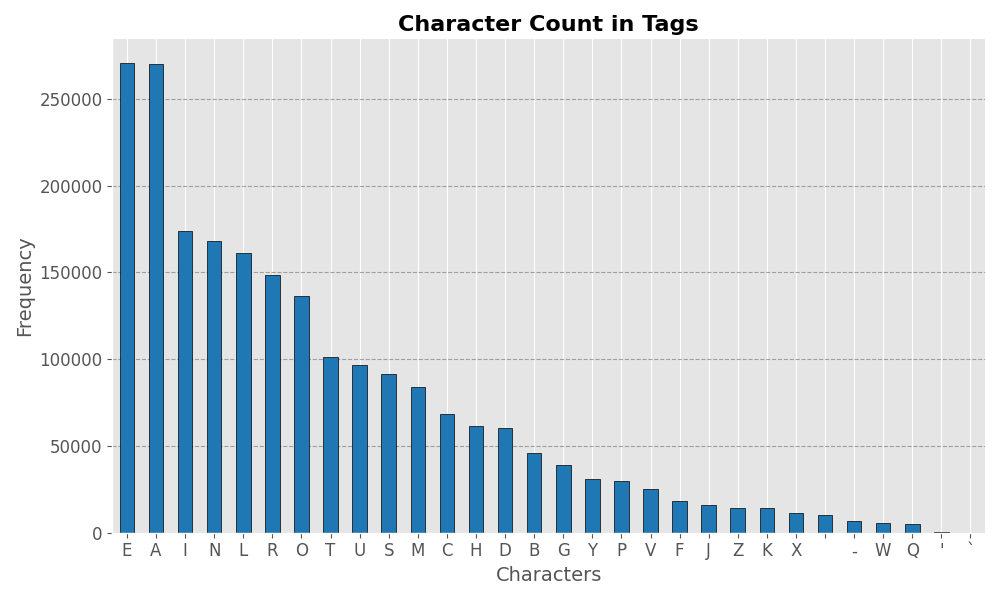
\includegraphics[width=0.65\linewidth]{character_count.png}
		\caption{Character presence in dataset.}
		\label{fig:char_freq}
	\end{figure}
	
	After detecting this potential issue, we decided to still use this dataset since even if some characters have a relatively small count, it is still a high absolute value. We then proceeded to take a look to the dataset as shown in table \ref{tab:dataset}; the model will later access these images with the function \texttt{download\_dataset\_base\_path}.
	
	\begin{table}[h]
		\centering
		\begin{tabular}{|c|c|c|}
			\hline
			\# & FILENAME & IDENTITY \\
			\hline
			0 & TRAIN\_00001.jpg & BALTHAZAR \\
			\hline
			1 & TRAIN\_00002.jpg & SIMON \\
			\hline
			2 & TRAIN\_00003.jpg & BENES \\
			\hline
			3 & TRAIN\_00004.jpg & LA LOVE \\
			\hline
			4 & TRAIN\_00005.jpg & DAPHNE \\
			\hline
		\end{tabular}
		\caption{Training set head.}
		\label{tab:dataset}
	\end{table}
	
	\newpage
	
	\subsection{Variables and Hyperparameters}
	After choosing and exploring the dataset, we decided to use the \textit{Keras} and \textit{TensorFlow} frameworks in order to build our neural network. To start with, we imported the necessary libraries in our script, then we took on setting up the constants and hyperparameters for the model as shown in table \ref{tab:hyperparams}. Next, we defined some global dynamic variables that will have importance during data preprocessing such as filenames and model callbacks.
	
	\begin{table}[h]
		\centering
		\begin{tabular}{|l|p{8cm}|}
			\hline
			Hyperparameter/Constant & Value \\
			\hline
			dataset\_url & \url{https://www.kaggle.com/api/v1/datasets/download/ssarkar445/handwriting-recognitionocr} \\
			\hline
			img\_height & 60 \\
			\hline
			img\_width & 128 \\
			\hline
			input\_c & 1 \\
			\hline
			epochs & 200 \\
			\hline
			initial\_learning\_rate & 0.001 \\
			\hline
			batch\_size & 1024 \\
			\hline
			AUTOTUNE & \texttt{tf.data.AUTOTUNE} \\
			\hline
			empty\_prediction\_penalty & 50.0 \\
			\hline
		\end{tabular}
		\caption{Definition of hyperparameters and constants.}
		\label{tab:hyperparams}
	\end{table}
	
	\subsection{Metric} \label{subsec:metric}
	We defined a custom class to compute the \textbf{Character Error Rate} (CER) as the metric to evaluate the performance of our model. This value measures the number of character-level errors (insertions, deletions, substitutions) made by the model when predicting a character sequence and comparing it to the target.
	
	This class includes three key fields: \texttt{cer\_accumulator}, \texttt{num\_samples}, and \texttt{actual\_padding\_token}. When the metric is updated, the \texttt{ctc\_greedy\_decoder} converts the model's output logits (which represent the probability distribution over characters at each time step) into a predicted sequence by selecting the most likely token at each time step. After decoding, padding is removed from the ground truth (label) and the edit distance is calculated. CTC decoding is necessary for alignment-free predictions, especially since the input and output length may differ.
	
	The total edit distance is added to \texttt{cer\_accumulator}, and the number of samples in the current batch is added to \texttt{num\_samples}. The final CER is calculated by dividing the accumulated edit distances by the total number of characters in the target labels.
	
	To discourage behavior such as the model defaulting to blank outputs, we introduced a penalty for empty predictions. This encourages the model to attempt meaningful outputs.
	
	\subsection{Data preprocessing}
	In order to access the data, we defined two functions: \texttt{download\_dataset\_base\_path}, and \texttt{get\_initial\-\_metadata\_from\_csv}. The first function extracts the dataset in a determined path that is returned, and the second function reads the dataset to retrieve important information such as all the characters present, the length of the biggest label, filenames, and their corresponding labels.
	
	For the \textit{TensorFlow} input pipeline, we use several functions to prepare image-label pairs for efficient model training. The \texttt{load\_and\_process\_image} function reads the image file as raw bytes, then decodes it into a grayscale tensor, resizes the image to a consistent height and width using padding to preserve aspect ratio, and normalizes the pixel values from a [0, 255] range into [0, 1]. It returns the processed image with the raw label string and its length. 
	
	The \texttt{vectorize\_label\_tf} function splits the label into characters and converts them into an integer, then pads the sequence with a $-1$ token (required for batching variable-length sequences) to a fixed length and returns the padded label with the original length.
	
	Finally, the \texttt{create\_tf\_dataset} function creates the dataset that will be used for the \textit{TensorFlow} model, using the previous helper functions to map the original dataset, preparing it for model use. Then the processed data is cached into the memory.
	
	\subsection{Model class} \label{subsec:model_class}
	For our model we define a custom class \textbf{CTCOCRModel} that creates the neural network and manages the metric explained in section \ref{subsec:metric}. This class implements custom \texttt{train\_step} and \texttt{test\_step} methods allowing control over how loss is computed, direct integration with the metric, and dynamic loss computation with sparse tensors to support variable-length labels. \textbf{CTC Loss} is used since it allows training without requiring aligned input and output sequences, which is ideal for OCR tasks where the position of characters in the image isn't strictly aligned with output positions.
	
	\subsubsection{Network Architecture}
	The implemented network has a \textbf{hybrid architecture} that combines a convolutional network (CNN) with a bidirectional long short-term memory network (BiLSTM), as shown in figure \ref{fig:net_architecture}.
	
	The model begins with a convolutional block composed of convolution and pooling layers that extract spatial features from the input image, then a reshape layer converts the 3D feature map output from the CNN into a sequence of vectors suitable for recurrent layers, next the fully connected dense layers refine the extracted features to allow more abstract representations, after that the dropout layer prevents overfitting by encouraging redundancy in learned features, subsequently the bidirectional LSTM layers process the sequence in both directions (figure \ref{fig:bilstm_process}), and finally the output dense layer outputs logits for each character class at each time step (position), making the output compatible with the Connectionist Temporal Classification (CTC) loss function.
	
	\begin{figure}[h]
		\centering
		\begin{subfigure}[b]{0.58\linewidth}
			\centering
			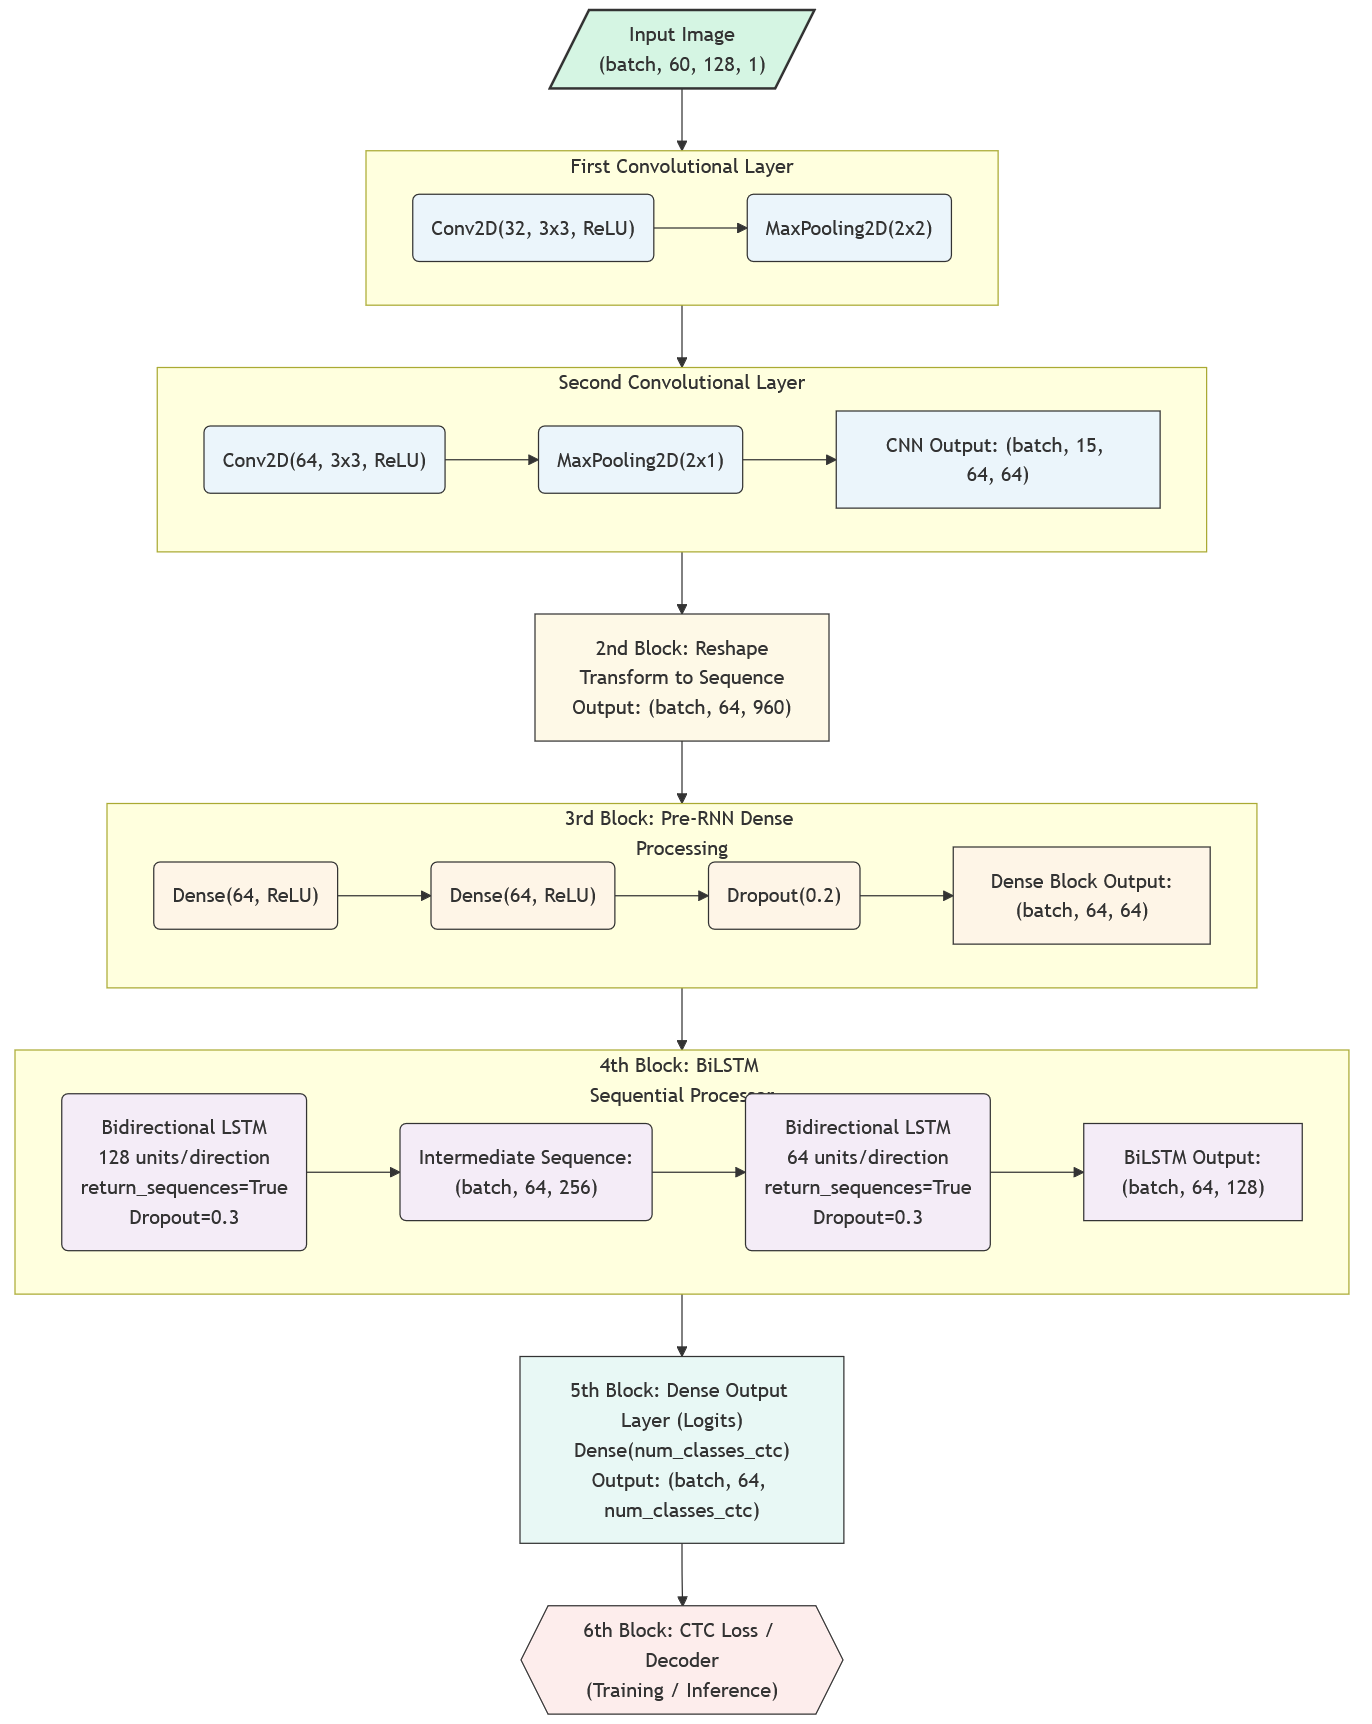
\includegraphics[width=\linewidth]{network_architecture_v2.png}
			\caption{Model's neural network architecture.}
			\label{fig:net_architecture}
		\end{subfigure}
		\hfill
		\begin{subfigure}[b]{0.38\linewidth}
			\centering
			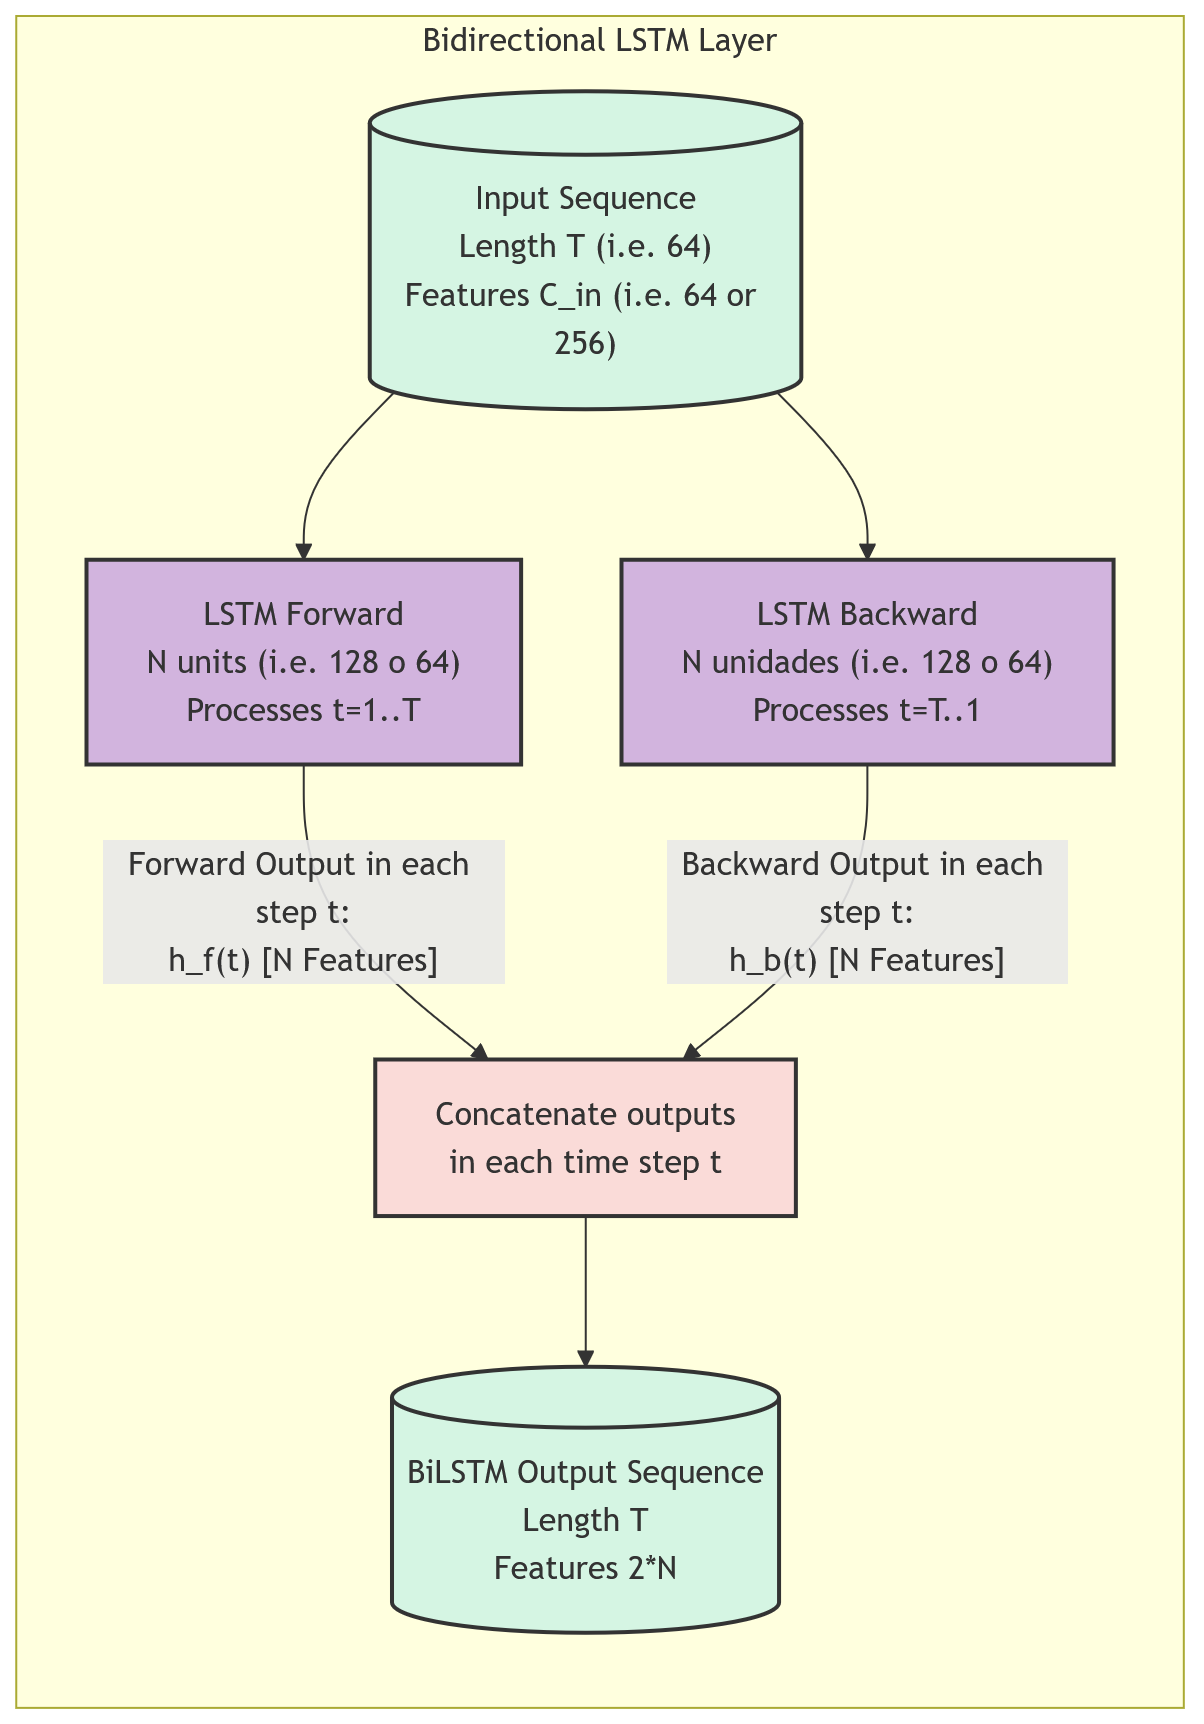
\includegraphics[width=\linewidth]{bilstm_process_v2.png}
			\caption{BiLSTM layer process.}
			\label{fig:bilstm_process}
		\end{subfigure}
		\caption{Neural network architecture and BiLSTM process.}
		\label{fig:combined}
	\end{figure}
	
	\newpage
	
	\subsection{Main Workflow and Model Configuration}
	The principal workflow is defined as follows:
	\begin{enumerate}
		\item Obtain metadata and image/tags pairs from the training dataset.
		\item Start the \texttt{StringLookup} object to map characters to integers.
		\item Create the \texttt{tf.data.Dataset} dataset that will actually be used to train, validate, and test the model.
		\item Calculate the number of classes for CTC and prediction length.
	\end{enumerate}
	
	The output of this cell block can be seen in table \ref{tab:vocab_params}. As shown, there are 33 different classes: 26 letters, and 1 character for back-tick, apostrophe, space, empty, unknown, and dash.
	
	\begin{table}[!h]
		\centering
		\begin{tabular}{|l|p{10cm}|}
			\hline
			\textbf{Parameter} & \textbf{Value} \\
			\hline
			Global Vocabulary (30 chars) & \texttt{-ABCDEFGHIJKLMNOPQRSTUVWXYZ` } \\
			\hline
			Max Label Length (from training set) & 34 \\
			\hline
			TF StringLookup Vocabulary (32 tokens) &
			\texttt{[''}, \texttt{[UNK]}, \texttt{' '}, \texttt{'''}, \texttt{'-'}, \texttt{'A'}, \texttt{'B'}, \texttt{'C'}, \texttt{'D'}, \texttt{'E'}, \texttt{'F'}, \texttt{'G'}, \texttt{'H'}, \texttt{'I'}, \texttt{'J'}, \texttt{'K'}, \texttt{'L'}, \texttt{'M'}, \texttt{'N'}, \texttt{'O'}, \texttt{'P'}, \texttt{'Q'}, \texttt{'R'}, \texttt{'S'}, \texttt{'T'}, \texttt{'U'}, \texttt{'V'}, \texttt{'W'}, \texttt{'X'}, \texttt{'Y'}, \texttt{'Z'}, \texttt{'`']} \\
			\hline
		\end{tabular}
		\caption{Character Vocabulary and Label Parameters.}
		\label{tab:vocab_params}
	\end{table}
	
	\newpage
	
	\subsection{Model Build and Loading a Model}
	To build the model we create an instance of the class defined in section \ref{subsec:model_class} with the parameters stated in table \ref{tab:model_config}. After the model is defined, it is compiled with an \textbf{Adam} optimizer with an initial learning rate of $0.1$, then it is built and the model summary can be consulted in table \ref{tab:architecture}.
	
	\begin{table}[!h]
		\centering
		\begin{tabular}{|l|c|}
			\hline
			\textbf{Parameter} & \textbf{Value} \\
			\hline
			Image height & 60 \\
			Image width & 128 \\
			Input channel & 1 \\
			Number of classes for CTC & 33 \\
			Prediction model output length & 64 \\
			\hline
		\end{tabular}
		\caption{Model Configuration Parameters.}
		\label{tab:model_config}
	\end{table}
	
	\begin{figure}[!h]
		\centering
		\begin{subfigure}[b]{0.75\linewidth}
			\centering
			\begin{tabular}{|l|c|r|}
				\hline
				\textbf{Layer (type)} & \textbf{Output Shape} & \textbf{Param \#} \\
				\hline
				\texttt{convolutional\_block (Sequential)} & (None, 15, 64, 64) & 18,816 \\
				\texttt{reshape\_to\_sequence (Reshape)} & (None, 64, 960) & 0 \\
				\texttt{dense (Dense)} & (None, 64, 64) & 61,504 \\
				\texttt{dense\_1 (Dense)} & (None, 64, 64) & 4,160 \\
				\texttt{dropout (Dropout)} & (None, 64, 64) & 0 \\
				\texttt{bidirectional (Bidirectional)} & (None, 64, 256) & 197,632 \\
				\texttt{bidirectional\_1 (Bidirectional)} & (None, 64, 128) & 164,352 \\
				\texttt{output\_logits (Dense)} & (None, 64, 33) & 4,257 \\
				\hline
			\end{tabular}
			\caption{Layer-wise architecture}
			\label{tab:architecture}
		\end{subfigure}
		
		\vspace{1em}
	
		\begin{subfigure}[b]{0.75\linewidth}
			\centering
			\begin{tabular}{|l|r|}
				\hline
				\textbf{Total parameters} & 450,721 (1.72 MB) \\
				\textbf{Trainable parameters} & 450,721 (1.72 MB) \\
				\textbf{Non-trainable parameters} & 0 (0.00 B) \\
				\hline
			\end{tabular}
			\caption{Parameter summary}
		\end{subfigure}
		
		\caption{Model Summary. Architecture and Parameter Counts.}
		\label{fig:model_summary}
	\end{figure}
	
	\subsubsection{Loading a previous model} \label{subsubsec:loading_model}
	Since we wanted to test the model every 300 epochs we trained on it, we designed a workflow that allows us to load a previous model to restart training on the actual number of epochs. This was essential for the development of the neural network because it let us see how the model was performing at a certain number of epochs and run some tests on the predictions.
	
	This workflow is mainly for previously trained models, but can also take only the weights to run tests on the testing dataset and visualize predictions.
	
	\subsection{Training}
	After the model is successfully built, it is trained on the training dataset for a certain number of epochs. Once training is complete, the model and weights are saved as files to allow future loading as explained in section \ref{subsubsec:loading_model}.
	
	The model is trained with the \textbf{CTC Loss} function and the \textbf{CER} metric. It also has two callbacks that implement techniques to increase the training efficiency: \texttt{EarlyStopping} to stop the training if \texttt{val\_loss} does not get better after 6 epochs, and \texttt{ReduceLROnPlateau} that decreases learning rate when the validation metric no longer reduces.
	
	\section{Previous Models}
	The initial model yielded extremely poor performance, likely due to inadequate training duration and suboptimal preprocessing. After some tweaks and fixes to the source code including the following:
	\begin{itemize}
		\item Changes in how data was loaded and processed.
		\item Adjustments in how the labels were vectorized and padded.
		\item The implementation of a personalized class for the model (as detailed in section \ref{subsec:model_class}).
		\item Tweaks to the CNN block output and the reshape layer.
		\item Fixes to the metric, resulting in the final version stated in section \ref{subsec:metric}.
		\item Add a class to the total number of classes for the model's output.
	\end{itemize}
	
	Despite these improvements, the performance remained below expectations, particularly with respect to the CER and validation loss. The comparison between said models is displayed in table \ref{tab:model_comp}.
	
	\begin{table}[!h]
		\centering
		\begin{tabular}{|c|c|c|}
			\hline
			Model Version & First & Second \\
			\hline
			Epochs & 100 & 100 \\
			\hline
			Learning rate & 0.001 & 0.0001 \\
			\hline
			Batch size & 1024 & 1024 \\
			\hline
			val\_loss & 727.3027 & 5.26555 \\
			\hline
			CER & N/A & 1.2292 \\
			\hline
		\end{tabular}
		\caption{Comparison between first two models.}
		\label{tab:model_comp}
	\end{table}
	
	\section{Results}
	After picking up the second model to restart training from where it was left off, we added 112 epochs and changed the learning rate to $0.001$. The resulting model is the final result of the article, it reached a validation loss of less than 5 per epoch, and a CER per epoch smaller than 1.2, as seen in figure \ref{fig:final_metrics}. Some of the made predictions over the test set are showcased in figure \ref{fig:model_pred}.
	
	\begin{figure}[h]
		\centering
		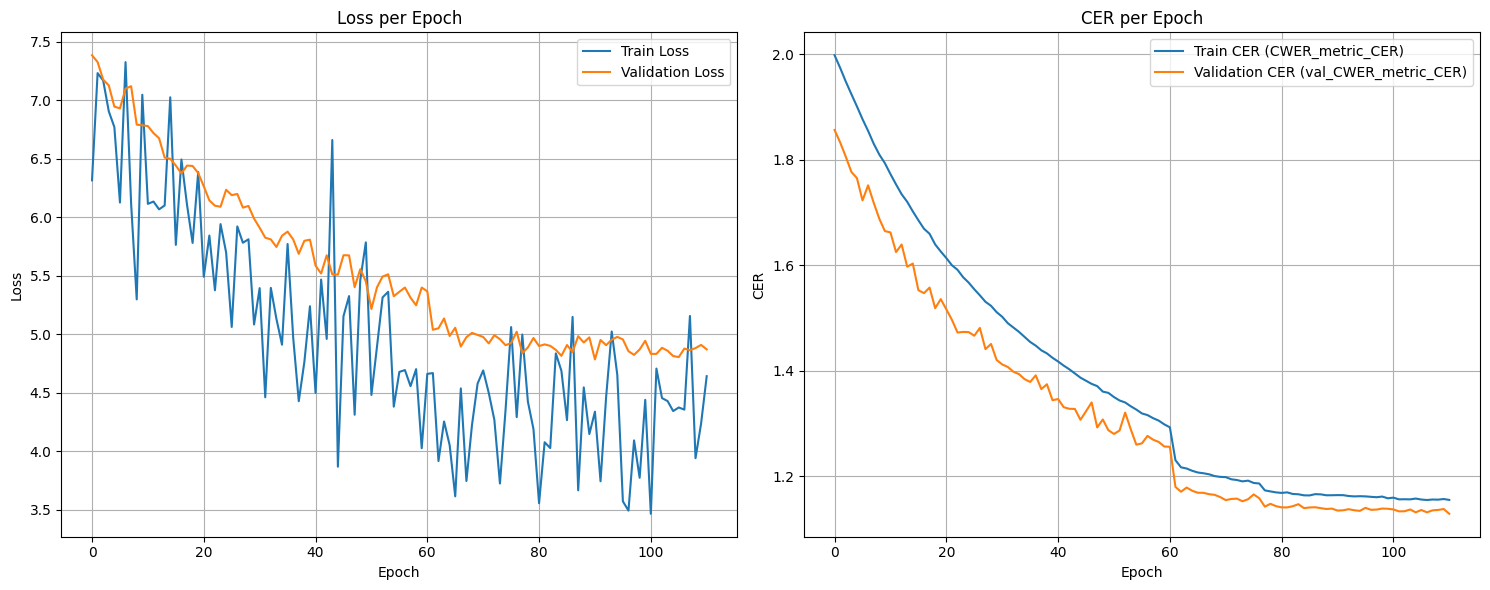
\includegraphics[width=\linewidth]{final_model_graphs.png}
		\caption{Metrics for the third model.}
		\label{fig:final_metrics}
	\end{figure}
	
	\begin{figure}[!h]
		\centering
		\begin{subfigure}[b]{0.45\linewidth}
			\centering
			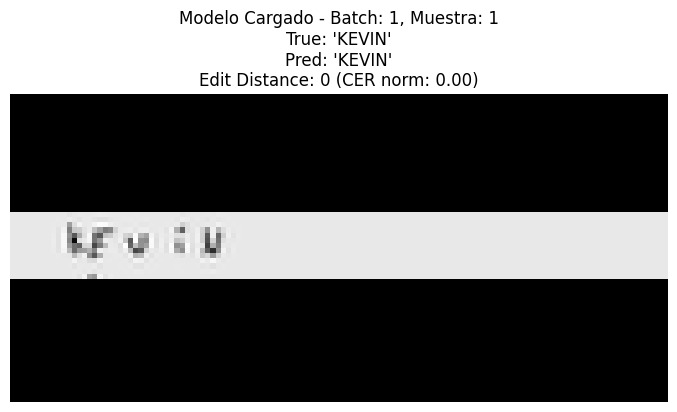
\includegraphics[width=\linewidth]{pred1.jpg}
		\end{subfigure}		
		\begin{subfigure}[b]{0.45\linewidth}
			\centering
			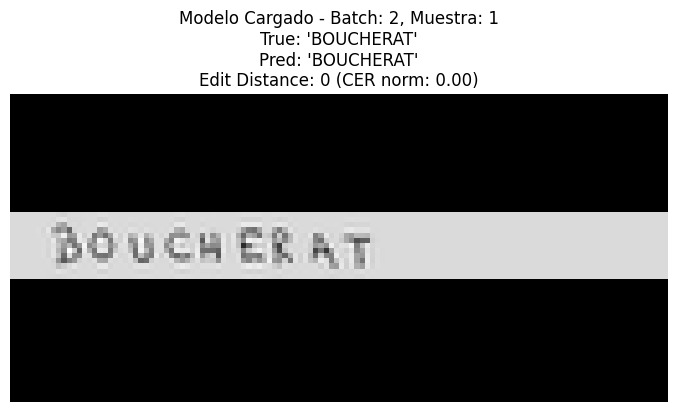
\includegraphics[width=\linewidth]{pred2.jpg}
		\end{subfigure}
		\begin{subfigure}[b]{0.45\linewidth}
			\centering
			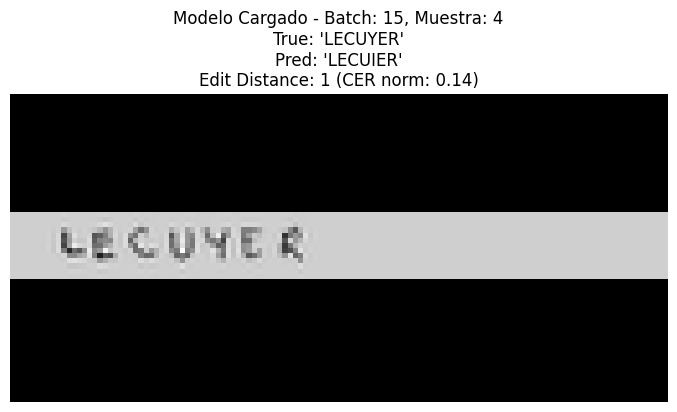
\includegraphics[width=\linewidth]{pred3.jpg}
		\end{subfigure}	
		\begin{subfigure}[b]{0.45\linewidth}
			\centering
			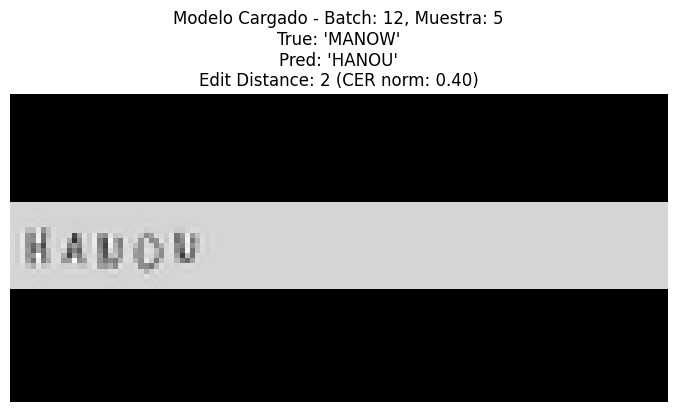
\includegraphics[width=\linewidth]{pred4.jpg}
		\end{subfigure}	
		\caption{Predictions made by the model.}
		\label{fig:model_pred}
	\end{figure}
	
	\newpage
	
	\section{Conclusions}
	
	The results demonstrate that the model is capable of effectively predicting names with a relatively high degree of accuracy. This indicates that the current architecture and training regimen are sufficient for capturing the underlying patterns in the dataset. However, there remains room for further improvement and refinement.
	
	For instance, extending the training process by an additional 100 epochs may allow the model to converge more fully and potentially achieve better generalization. Additionally, increasing the number of filters in the convolutional layers could enable the network to learn more complex and nuanced features from the input data. These adjustments could lead to enhanced performance, particularly in edge cases or less common naming patterns.
	
	Nonetheless, implementing such modifications goes beyond the scope and intent of this article, which primarily aimed to explore the feasibility of using this specific neural architecture for name prediction tasks. Future work may consider these directions in order to further optimize and expand the capabilities of the model.
	
	\bigskip
	
	\bibliographystyle{apalike-ejor}
	\bibliography{entregable5_bib}
	
\end{document}